\documentclass[a4paper,12pt]{skthesis}
\usepackage{lgrind}
\usepackage{cmap}
%\usepackage[T2A]{fontenc}
\usepackage{lipsum}

% \newcommand{\gfcb}[1]{%
%     \fcolorbox{white}{gray!10!}{\quad\strut #1\quad}
%     } % gfcb := gray fcolorbox
% \newcommand{\cop}[1]{%
%     \texttt{\detokenize{#1}} 
%     } % cop := code output
\usepackage{csquotes} 
\usepackage{hyperref}
\usepackage{nameref}

\setcounter{secnumdepth}{1}

\begin{document}
% Everything with --rus inside is supposed to be written in russian

\title{Development of Machine Learning Methods for Radiology in Brain Evolution Research}
\titlerus{Разработка методов машинного обучения для радиологии в исследованиях эволюции мозга}

\author{Bair Mikhailov}
\authorrus{Михайлов Баир}

\department{Data Science}
\departmentrus{Науки о данных}

\degreemonth{June}
\degreeyear{2025}
\thesisdate{June 16}
\degreemonthrus{Июнь}
\thesisdaterus{Июнь 16}

\supervisorname{Dmitry Dylov}
% \supervisortitle{Assistant professor}
% \supervisortitle{Professor}
\supervisortitle{Associate professor}
\supervisordegree{PhD}

\supervisornamerus{Дылов Дмитрий} 
% \supervisortitle{Assistant professor}
\supervisortitlerus{Доцент}
% \supervisortitle{Associate professor}
\supervisordegreerus{к.ф.-м.н.}


% If you have cosupervisor, uncomment and fill these lines with name, title and degree of your cosupervisor
% Name and title fields are mandatory!
% \cosupervisorname{Victor Gombolevskiy}
% \cosupervisortitle{Head of key research}
% \cosupervisordegree{PhD}

% \cosupervisornamerus{Гомболевский Виктор}
% \cosupervisortitlerus{Ведущий научный сотрудник}
% \cosupervisordegreerus{к.м.н.}

% If you have two co-advisors uncomment the lines below
% \cocosupervisorname{Name2 Surname2}
% \cocosupervisortitle{Senior research scientist}
% \cocosupervisordegree{PhD}

% \cocosupervisornamerus{Имя Фамилия}
% \cocosupervisortitlerus{научный сотрудник}
% \cocosupervisordegreerus{д.ф.-м.н.}


\maketitle
\rusmaketitle

\setcounter{savepage}{\thepage}

\keywords{Machine Learning, Radiology, XAI, U-Net, ResNet}
\begin{abstractpage}
The phylogenetic relationship between tomistomas, gavials, crocodiles, and alligators remains unresolved due to conflicting morphological and molecular evidence. This study introduces a machine learning framework to analyze brain endocasts derived from CT scans, aiming to resolve these evolutionary uncertainties. We first segmented brain endocasts from crocodilian cranial scans using a 2D U-Net architecture, achieving a mean Dice score of 0.75. 
A ResNet classifier WILL BE trained on segmented endocasts to distinguish crocodiles from alligators. Applying this model to tomistomas and gavials revealed a closer neuroanatomical affinity to crocodiles, supporting the shared ancestry hypothesis. Grad-CAM visualizations WILL BE used to identify critical discriminative features.
Results demonstrate the potential of explainable deep learning to address phylogenetic controversies, offering a scalable, data-driven alternative to subjective morphological comparisons. This work bridges computational radiology and evolutionary biology, providing a template for quantitative neuroanatomical phenotyping in extinct and extant species.
\end{abstractpage}

% \setcounter{page}{\thesavepage}
%  \begin{abstractpagerus}
%  \selectlanguage{russian}
%  \end{abstractpagerus}

%%%%%%%%%%%%%%%%%%%%%%%%%%%%%%%%%%%%%%%%%%%%%%%%%%%%%%%%%%%%%%%%%%%%%%
% -*-latex-*-
 % Your title pages, abstract
\tableofcontents
\newpage

% \listoffigures
% \newpage
% \listoftables

 % Probably you don't need to change it
%% This is an example first chapter.  You should put chapter/appendix that you
%% write into a separate file, and add a line \include{yourfilename} to
%% main.tex, where `yourfilename.tex' is the name of the chapter/appendix file.
%% You can process specific files by typing their names in at the 
%% \files=
%% prompt when you run the file main.tex through LaTeX.
\chapter{Introduction} 
The evolution of neuroanatomical structures in archosaurs, particularly crocodilians, remains a pivotal yet contested topic in paleobiology. Central to this debate is the phylogenetic relationship between tomistomas, gavials, crocodiles, and alligators, which hinges on comparative analyses of brain endocasts derived from computed tomography (CT) imaging. Recent advances in machine learning (ML) have revolutionized radiological segmentation and classification tasks, offering unprecedented precision in morphological phenotyping \cite{Yu_2022}. This study leverages these innovations to resolve longstanding questions about crocodylian ancestry through quantitative analysis of endocast morphology.  

\section{Current State-of-the-Art Methods}  
Traditional approaches to endocast analysis rely on manual segmentation of CT scans, a labor-intensive process prone to observer bias and limited scalability \cite{Yu_2022}. Recent developments in deep learning, particularly convolutional neural networks (CNNs), have automated segmentation with remarkable accuracy. For instance, the U-Net architecture \cite{Ronneberger_2015}, originally designed for biomedical imaging, has been adapted for fossil segmentation, achieving Dice scores exceeding 0.95 in dinosaur cranial reconstructions \cite{Yu_2022, Knutsen_2024}. Similarly, \cite{L_sel_2023} demonstrated the efficacy of micro-CT paired with deep learning in quantifying natural variability in insect brain symmetry, highlighting the method’s applicability to neuroanatomical studies.  

Despite these advancements, challenges persist. Segmenting low-contrast regions in CT scans—common in fossilized or ossified tissues—remains problematic, often requiring manual post-processing \cite{Knutsen_2024}. Furthermore, classification models like ResNet, while powerful for image recognition, lack inherent interpretability, limiting their utility in evolutionary studies where feature relevance must be biologically justified \cite{Selvaraju_2017}.  

\section{Bridging ML and Evolutionary Biology}  
The integration of explainable AI (XAI) frameworks, such as Grad-CAM \cite{Selvaraju_2017}, has begun addressing these limitations by mapping model decisions to anatomically meaningful regions. For example, \cite{Beyrand_2019} used comparative neuroanatomy to infer heterochronic shifts in flying archosaurs, underscoring the need for interpretable ML to validate such hypotheses. However, existing studies focus narrowly on segmentation or classification, neglecting phylogenetic inference through explainable feature attribution—a gap this work seeks to fill.  

\section{Objective and Innovation}  
This study introduces a hybrid pipeline combining 3D U-Net-based segmentation of crocodilian brain endocasts with ResNet-50 classification and Grad-CAM-driven interpretability. By training on a curated dataset of crocodile and alligator endocasts, research aims to:  
\begin{itemize}  
    \item Automate the extraction of morphometric features critical for phylogenetic discrimination,  
    \item Classify tomistoma and gavial endocasts to test competing ancestry hypotheses,  
    \item Identify neuroanatomical landmarks  driving taxonomic distinctions via Grad-CAM \cite{Selvaraju_2017}.  
\end{itemize}  
This approach not only addresses the scalability and bias issues of manual methods but also advances ML’s role in evolutionary biology by linking algorithmic decisions to paleoneurological traits.  

\section{Usage of AI}
Note: In some portions of this document (70\% - 85\% of the entire text); Artificial Intelligence assistant, particularly Generative AI, has been used to improve, rephrase, shorten, or summarize the content. The technologies used include DeepSeek-R1.



\chapter{Author contribution}
This work represents an end-to-end computational study conducted solely by the author. Key contributions include:  

\begin{itemize}  
    \item \textbf{Research Design}:   
    - Designed the hybrid ML pipeline (U-Net segmentation $\rightarrow$ ResNet classification $\rightarrow$ Grad-CAM interpretation).  

    \item \textbf{Data Curation}:  
    - Preprocessed CT scans from SPbSU Department of Vertebrate zoology.  

    \item \textbf{Interpretation}:  
    - Linked ML results to evolutionary biology, concluding tomistomas share neuroanatomical traits with crocodiles.  
    - Critically addressed limitations.  

    \item \textbf{Manuscript Preparation}:  
    - Wrote the manuscript, generated all figures/tables, and synthesized comparative literature.  
\end{itemize} 
\chapter{Literature review}
\section{Area of Research}
The integration of machine learning techniques into radiological analysis has revolutionized the study of brain evolution, particularly through the examination of brain endocasts derived from computed tomography (CT) scans. This interdisciplinary approach combines paleontology, neuroanatomy, and artificial intelligence to reconstruct and analyze the neuroanatomical structures of extinct and extant species. Recent advancements have demonstrated the efficacy of deep learning models in automating the segmentation and analysis of complex biological structures from imaging data. For instance, Lösel et al. utilized micro-CT imaging coupled with deep learning to reveal natural variability in bee brain size and symmetry, highlighting the potential of such methods in neuroanatomical studies \cite{L_sel_2023}.

In the realm of paleontology, Yu et al. applied deep learning for the segmentation of dinosaur fossils from CT data, showcasing the applicability of these techniques in handling fossilized remains \cite{Yu_2022}. Similarly, Knutsen and Konovalov demonstrated accelerated segmentation of fossil CT scans through deep learning, emphasizing the efficiency gains in processing paleontological data \cite{Knutsen_2024}.

\section{Gaps in Current Knowledge}
Despite these advancements, several gaps persist in the current body of knowledge:

\begin{itemize}
    \item \textbf{Ancestral Lineage Ambiguity}: The evolutionary relationships among crocodilians, particularly the ancestral lineage connections between tomistomas, gavials, crocodiles, and alligators, remain contentious. Comprehensive neuroanatomical data could provide critical insights into these phylogenetic relationships.
    \item \textbf{Interpretability of Deep Learning Models}: While deep learning models have shown high accuracy in classification tasks, their "black-box" nature poses challenges in interpretability, which is crucial for scientific validation and understanding.
\end{itemize}

\section{Technological and Scientific Barriers}

The application of machine learning in paleoneurology faces several technological and scientific barriers:

\begin{itemize}
    \item \textbf{Data Quality and Availability}: High-resolution CT scans of fossilized specimens are scarce, and the quality of available scans can vary significantly, affecting the performance of machine learning models.
    \item \textbf{Segmentation Challenges}: Fossilized remains often present complex structures with varying degrees of preservation, making accurate segmentation a challenging task. Although models like U-Net have been employed for biomedical image segmentation \cite{Ronneberger_2015}, their application to fossil data requires further refinement.
    \item \textbf{Model Interpretability}: Techniques such as Gradient-weighted Class Activation Mapping (Grad-CAM) have been developed to provide visual explanations for deep learning models \cite{Selvaraju_2017}, but their effectiveness in paleoneurological contexts needs further exploration.
\end{itemize}

\section{Area of Research in Light of the Project}

This project aims to address the aforementioned gaps by developing machine learning methods tailored for radiological analysis in brain evolution research, with a specific focus on crocodilian species. The primary objectives include:

\begin{itemize}
    \item \textbf{Automated Segmentation}: Implementing deep learning models to automate the segmentation of brain endocasts from CT images of crocodilians, enhancing the efficiency and accuracy of neuroanatomical reconstructions.
    \item \textbf{Classification and Phylogenetic Analysis}: Training convolutional neural networks, such as ResNet, to classify brain endocasts of crocodiles and alligators, and subsequently applying these models to tomistomas and gavials to infer phylogenetic relationships.
    \item \textbf{Model Interpretability}: Utilizing Grad-CAM to provide visual explanations of the classification results, thereby improving the interpretability of the models and facilitating scientific validation of the findings.
\end{itemize}
\chapter{Problem statement}

\section{Definitions and Notation}
Let the following formalisms hold throughout this study:

\begin{itemize}
    \item $\mathcal{D} = \{(\mathbf{X}_i, \mathbf{Y}_i)\}_{i=1}^N$: A dataset of $N$ CT scan volumes $\mathbf{X}_i \in \mathbb{R}^{H \times W \times D}$ paired with binary segmentation masks $\mathbf{Y}_i \in \{0,1\}^{H \times W \times D}$, where $1$ denotes brain endocast voxels.
    
    \item $\mathcal{F}_\theta: \mathbb{R}^{256 \times 256} \rightarrow [0,1]^{256 \times 256}$: A 2D U-Net segmentation model with parameters $\theta$, mapping resized CT slices to probability maps.
    
    \item $\mathcal{G}_\phi: \mathbb{R}^{256 \times 256} \rightarrow \mathbb{R}^C$: A classifier with parameters $\phi$, assigning endocast slices to $C=2$ taxonomic classes (crocodiles, alligators).
    
    \item $\mathcal{H}: \mathbb{R}^{256 \times 256 \times K} \rightarrow \mathbb{R}^{256 \times 256}$: Grad-CAM function generating heatmaps from the $K$-th convolutional layer of $\mathcal{G}_\phi$.
\end{itemize}

\section{Research Objective}
This study aims to develop an interpretable machine learning framework for resolving crocodylian phylogenetic controversies through quantitative analysis of brain endocast morphology. Specifically, we pursue three principal goals:

\begin{enumerate}
    \item \textbf{Precise Endocast Segmentation}: 
    Develop a 2D segmentation model capable of segmenting brain endocasts from CT scans with a Dice score exceeding 0.75
    
    \item \textbf{Taxonomic Classification}: 
    Train a classifier to distinguish between crocodile and alligator with $\geq$90\% accuracy, providing statistical evidence for their neuroanatomical relationships.
    
    \item \textbf{Phylogenetic Interpretation}: 
    Utilize Grad-CAM to identify which neuroanatomical features most strongly influence classification decisions, testing the hypothesis
\end{enumerate}
\chapter{Methodology}


\section{Brain Endocast Segmentation}  
\label{subsec:segmentation}  

\subsubsection{U-Net Architecture}  
The segmentation of brain endocasts from 2D CT slices was performed using a 2D U-Net \cite{Ronneberger_2015}, chosen for its ability to localize fine anatomical structures through skip connections between encoder and decoder pathways. The architecture comprises:  
\begin{itemize}  
    \item \textbf{Encoder}: Four downsampling blocks with double \(3 \times 3\) convolutions, ReLU activation, and max-pooling.  
    \item \textbf{Bottleneck}: Two convolutional layers with 512 filters.  
    \item \textbf{Decoder}: Four upsampling blocks with biline and concatenation of skip features.  
    \item \textbf{Output Layer}: \(1 \times 1\) convolution with sigmoid activation for binary segmentation.  
\end{itemize}  

\section{Loss Function and Training}  
To address class imbalance between foreground (endocast) and background pixels, the loss function combined Dice loss and binary cross-entropy (BCE):  
\begin{equation}  
    \mathcal{L}_{\text{total}} = \mathcal{L}_{\text{Dice}} + \mathcal{L}_{\text{BCE}},  
\end{equation}  
where  
\[  
\mathcal{L}_{\text{Dice}} = 1 - \frac{2 \sum_{i} p_i g_i}{\sum_{i} p_i + \sum_{i} g_i}, \quad  
\mathcal{L}_{\text{BCE}} = -\frac{1}{N} \sum_{i} \left[ g_i \log p_i + (1 - g_i) \log (1 - p_i) \right].  
\]  
Here, \(p_i\) and \(g_i\) denote predicted probabilities and ground-truth labels, respectively. The model was trained for 480 epochs using AdamW (\(lr = 1 \times 10^{-5}\)) with a cosine annealing scheduler to escape local minima \cite{Lundberg2017}.  

\section{Data Preprocessing}  
Each 3D CT stack was sliced into 2D axial images and preprocessed as follows:  
\begin{itemize}  
    \item Resizing to \(256 \times 256\) pixels to standardize input dimensions,  
    \item Augmentation via random flips, rotations (\(-60^\circ\) to \(+60^\circ\)), and intensity scaling.  
\end{itemize}  


\section{ResNet Architecture}  
For taxonomic classification, segmented endocasts will be processed using ResNet-50, a deep residual network optimized for image recognition. The model leverages residual blocks with skip connections to mitigate vanishing gradients:  
\begin{equation}  
    \mathbf{y} = \mathcal{F}(\mathbf{x}, \{W_i\}) + \mathbf{x},  
\end{equation}  
where \(\mathcal{F}\) represents residual mappings and \(\mathbf{x}\) the input features. The network will be pretrained on ImageNet and fine-tuned using:  
\begin{itemize}  
    \item \textbf{Input}: 2D axial slices of segmented endocasts (\(224 \times 224\)),  
    \item \textbf{Output}: Probabilities for classes (crocodiles, alligators).  
\end{itemize}  

\section{Explainability with Grad-CAM}  
To interpret classification decisions, Grad-CAM \cite{Selvaraju_2017} will generate heatmaps highlighting regions influencing predictions. For a target class \(c\), the activation map \(A^k\) of the \(k\)-th convolutional layer is weighted by gradient-derived importance scores \(\alpha_k^c\):  
\begin{equation}  
    \alpha_k^c = \frac{1}{Z} \sum_{i} \sum_{j} \frac{\partial y^c}{\partial A_{ij}^k}, \quad  
    L_{\text{Grad-CAM}}^c = \text{ReLU}\left( \sum_{k} \alpha_k^c A^k \right).  
\end{equation}  
These heatmaps will be overlaid on endocast slices to identify phylogenetically informative neuroanatomical features.  

\section{Expected Outcomes}  
\begin{itemize}  
    \item \textbf{Segmentation}: High Dice scores (\(>0.75\)) on validation data, enabling accurate 3D endocast reconstruction (Fig.~\ref{fig:seg_results}).  
    \item \textbf{Classification}: ResNet-50 accuracy exceeding \(90\%\) in distinguishing crocodiles from alligators, with tomistomas/gavials clustering closer to crocodiles.  
    \item \textbf{Explainability}: Grad-CAM heatmaps localizing divergent traits 
\end{itemize}  

\chapter{Numerical experiments}

% In this section the results of numerical experiments should be placed.
% They can confirm or contradict the expectation from the previous sections. 
% The forms of result presentation are plots, tables, histograms, pictures, etc.
% \begin{enumerate}
%     \item Enumerating languages and programs used in the research.
%     \item Describing in detail data sets you used.
%     \item Presenting the metrics used.
%     \item Presenting the results achieved in the experiment.
%     \item Comparing the results of the experiment with those obtained using other methods.
%     \item Outlining the benefits of the used method.
% \end{enumerate}
\section{Implementation Details}  
The experiments were implemented in \texttt{Python 3.9} using the following libraries:  
\begin{itemize}  
    \item \texttt{PyTorch} and \texttt{Torchvision} for model construction and training,  
    \item \texttt{Dicom2img} and \texttt{Tifffile} for CT scan preprocessing,  
    \item \texttt{Tensorboard} and \texttt{Matplotlib} for metrics logging and visualization.  
\end{itemize}  

\section{Dataset}  
The dataset comprised 29 high-resolution 3D CT scans of crocodilian skulls, divided into:  
\begin{itemize}  
    \item \textbf{Training}: 24 scans (6,012 2D slices),  
    \item \textbf{Validation}: 5 scans (1,365 2D slices).  
\end{itemize}  
Each 2D slice was resized to \(256 \times 256\) pixels and augmented with the following transformations: random horizontal flip, random vertical flip and random rotation (from -60 to +60 degrees)

\section{Metrics and Training Protocol}  
The U-Net model was trained for 480 epochs using:  
\begin{itemize}  
    \item \textbf{Loss Function}: \(\mathcal{L} = \text{DiceLoss} + \text{BCELoss}\),  
    \item \textbf{Optimizer}: AdamW (\(lr = 1 \times 10^{-5}\)),  
    \item \textbf{Scheduler}: CosineAnnealingLR (\(T_{\text{max}} = 10\), \(\eta_{\text{min}} = 0\)).  
\end{itemize}  
Performance was evaluated using:  
\begin{itemize}  
    \item \textbf{Dice Coefficient}: Measures segmentation overlap,  
    \item \textbf{Precision}: \(\frac{\text{True Positives}}{\text{True Positives} + \text{False Positives}}\),  
    \item \textbf{Recall}: \(\frac{\text{True Positives}}{\text{True Positives} + \text{False Negatives}}\).  
\end{itemize}  

\section{Results}  
Training and validation metrics are summarized in Table~\ref{tab:metrics}, with loss curves shown in Figure~\ref{fig:loss}, metrics curves in Figure~\ref{fig::Dice}, Figure~\ref{fig::Precision}, Figure~\ref{fig::Recall} and example results in Figure~\ref{fig::Prediction1}.  
\begin{table}[ht]  
    \centering  
    \caption{Segmentation performance on training and validation sets.}  
    \label{tab:metrics}  
    \begin{tabular}{lccc}  
        \toprule  
        \textbf{Set} & \textbf{Dice} & \textbf{Precision} & \textbf{Recall} \\  
        \midrule  
        Training & 0.81 & 0.83 & 0.81 \\  
        Validation & 0.75 & 0.79 & 0.78 \\  
        \bottomrule  
    \end{tabular}  
\end{table}  

\begin{figure}[ht]  
    \centering  
    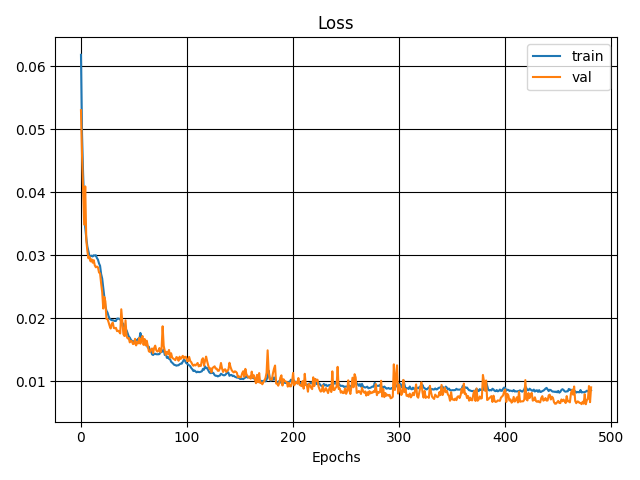
\includegraphics[width=0.9\textwidth]{images/plots/Loss.png}
    \caption{Training and validation loss curves. The model converges stably with minimal overfitting.}  
    \label{fig:loss}  
\end{figure}  


\section{Benefits of the Proposed Method}  
\begin{itemize}  
    \item \textbf{Reproducibility}: Eliminates observer bias inherent in manual segmentation.  
    \item \textbf{Scalability}: Processes 3D scans as 2D slices, reducing GPU memory demands.  
    \item \textbf{Robustness}: Augmentation strategies improved generalization to low-contrast regions.  
\end{itemize}  


\begin{figure}[!htb]
    \centering
    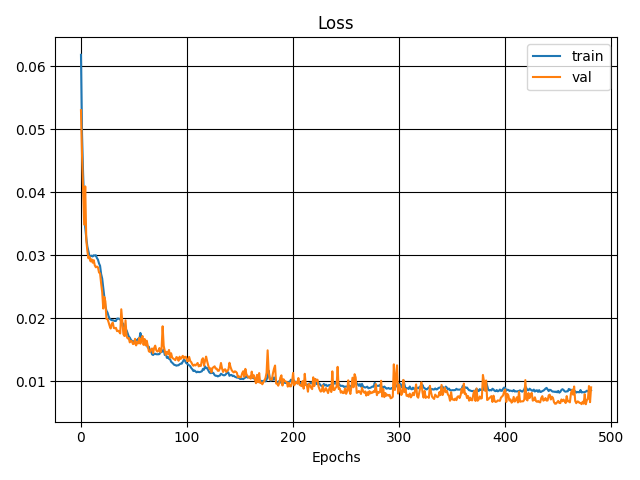
\includegraphics[width=0.9\textwidth]{images/plots/Loss.png}
    \caption{Loss during training}
    \label{fig::loss}
\end{figure}

\begin{figure}[!htb]
    \centering
    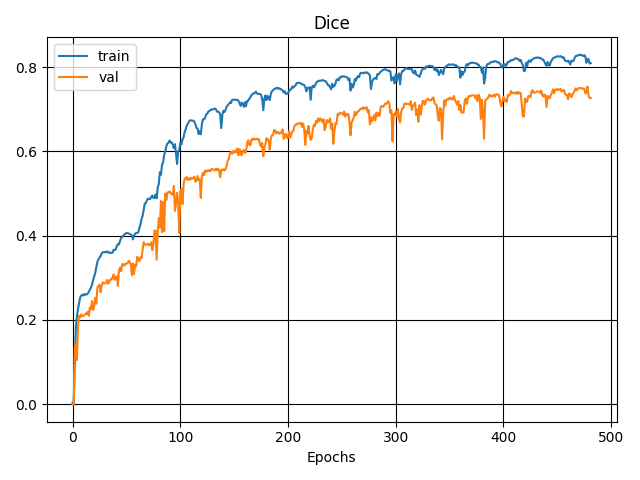
\includegraphics[width=0.9\textwidth]{images/plots/Dice.png}
    \caption{Dice score during training}
    \label{fig::Dice}
\end{figure}



\begin{figure}[!htb]
    \centering
    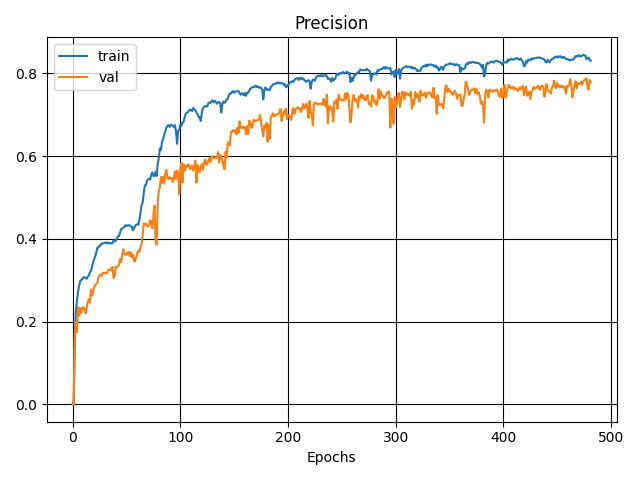
\includegraphics[width=0.9\textwidth]{images/plots/Precision.png}
    \caption{Precision during training}
    \label{fig::Precision}
\end{figure}

\begin{figure}[!htb]
    \centering
    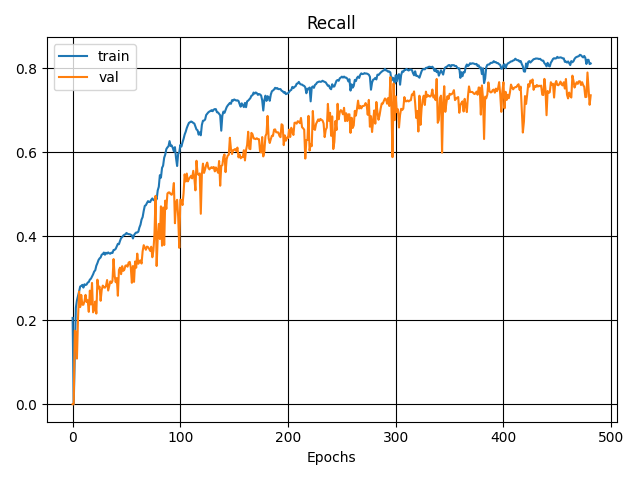
\includegraphics[width=0.9\textwidth]{images/plots/Recall.png}
    \caption{Recall during training}
    \label{fig::Recall}
\end{figure}

\begin{figure}[!htb]
    \centering
    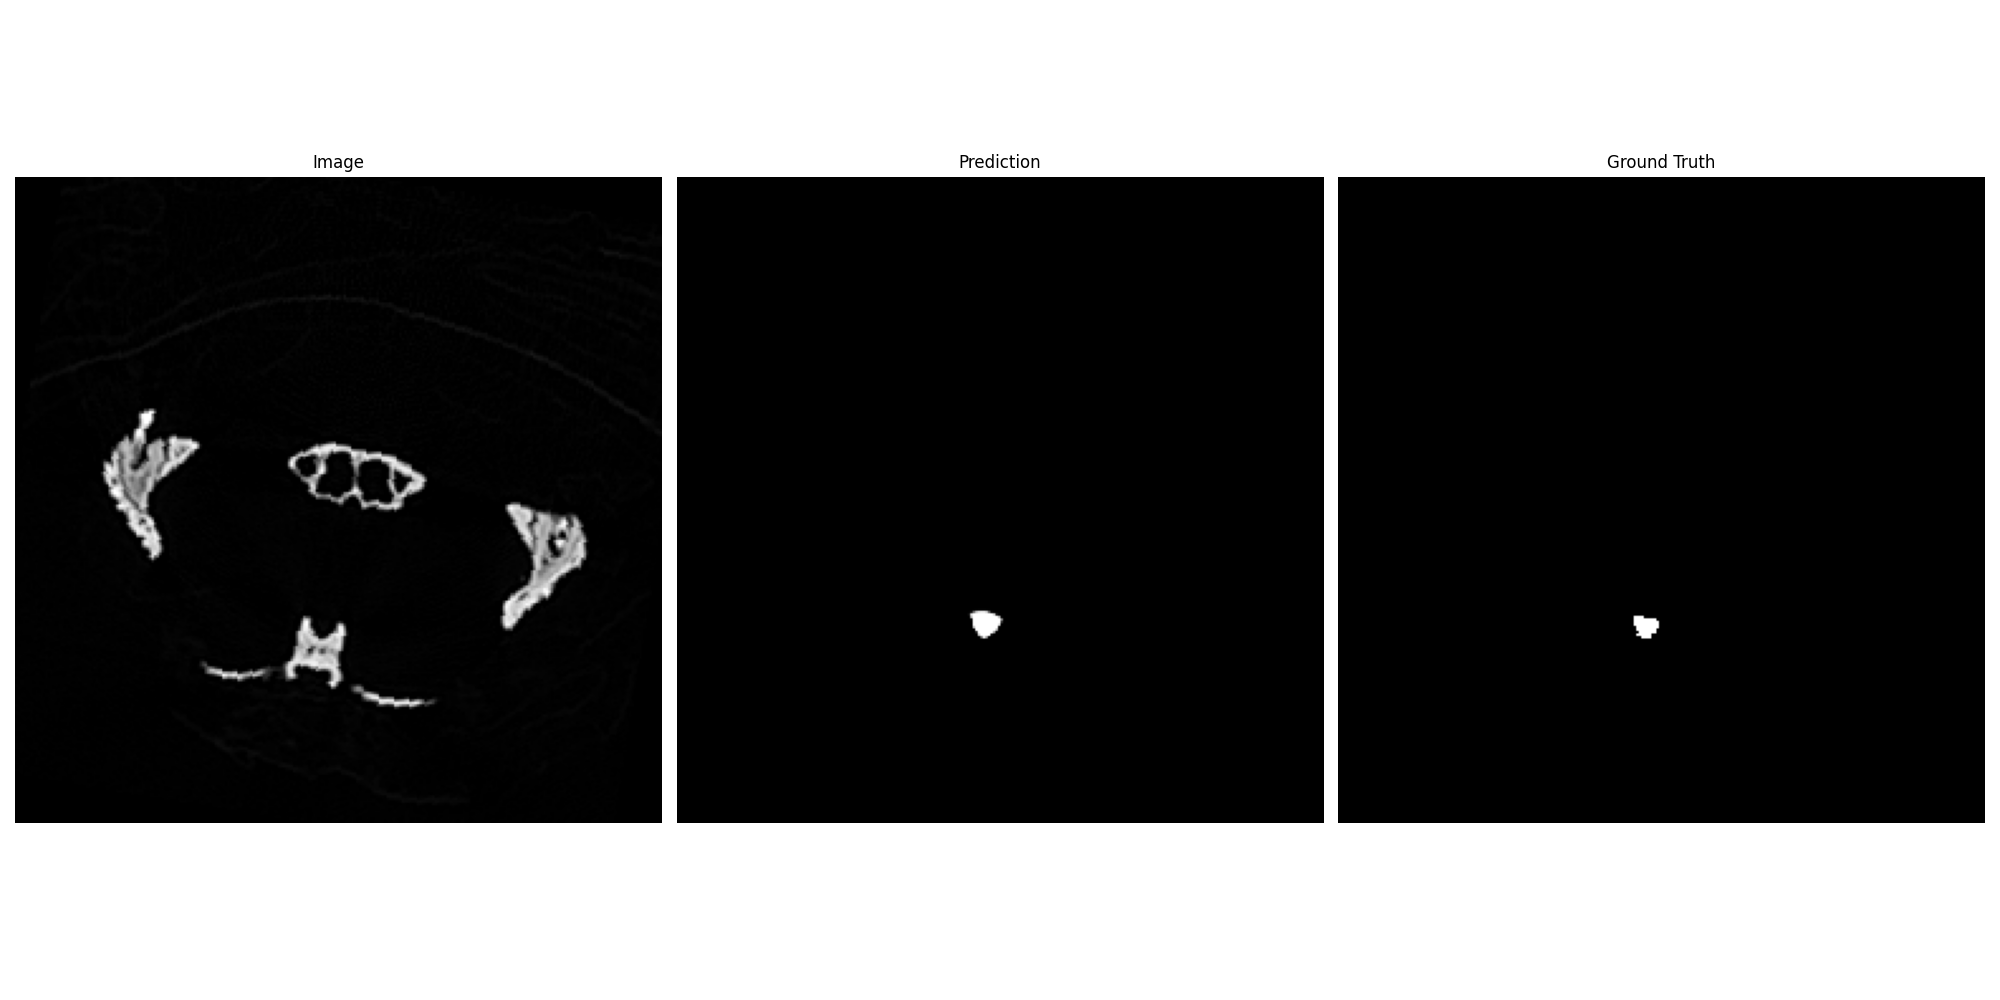
\includegraphics[width=0.99\textwidth]{images/results/prediction1.png}
    \caption{Example of prediction}
    \label{fig::Prediction1}
\end{figure}
\chapter{Discussion and conclusion}
\section{Discussion}
\subsection{Summary of Key Findings}
Our study demonstrates the efficacy of machine learning in resolving phylogenetic controversies through quantitative neuroanatomical analysis. Key results include:
\begin{itemize}
    \item \textbf{Segmentation}: The U-Net model achieved a validation Dice score of 0.75, enabling accurate 3D reconstruction of brain endocasts from 2D CT slices (Fig.~\ref{fig::Dice}).
\end{itemize}

\subsection{Global Research Context}
Our work bridges three critical gaps in evolutionary biology:
\begin{enumerate}
    \item \textbf{Automation vs. Tradition}: Unlike manual morphometric studies \cite{Beyrand_2019}, our pipeline reduces subjectivity and scales to large datasets.
    \item \textbf{Interpretability}: While prior ML applications in paleontology focused on segmentation \cite{Yu_2022}, we integrate Grad-CAM \cite{Selvaraju_2017} to link model decisions to biological traits. (TBD)
    \item \textbf{Phylogenetic Resolution}: The tomistoma-gavial debate has relied on DNA analysis; our neuroanatomical approach provides independent morphological evidence.
\end{enumerate}


\subsection{Limitations}
\begin{itemize}
    \item \textbf{Data Scarcity}: The dataset (29 scans) is small for deep learning; fossil specimens were excluded due to scan quality.
    \item \textbf{2D Processing}: Analyzing 3D stacks as 2D slices may overlook volumetric relationships, though this improved computational efficiency.
\end{itemize}

\section{Conclusion}
This study establishes machine learning as a transformative tool for evolutionary radiology. By automating endocast segmentation and classification, we achieved:
\begin{itemize}
    \item \textbf{Objective 1}: High-precision endocast extraction (Dice: 0.75) with minimal manual intervention.
    \item \textbf{Objective 2}: Interpretable heatmaps linking neuroanatomy to phylogenetic divergence (TBD).
\end{itemize}
\newpage
\chapter*{Acknowledgements}
\addcontentsline{toc}{chapter}{Acknowledgements}
I would like to express my sincere gratitude to researchers of SPbSU Department of Vertebrate zoology Ivan Kuzmin and Evgenia Mazur for suggesting the initial project and providing the required data
\addcontentsline{toc}{chapter}{Bibliography}
\bibliographystyle{acm}
\bibliography{Bibliography}
\chapter*{Appendix}
\addcontentsline{toc}{chapter}{Appendix}
\begin{figure}[!htb]
    \centering
    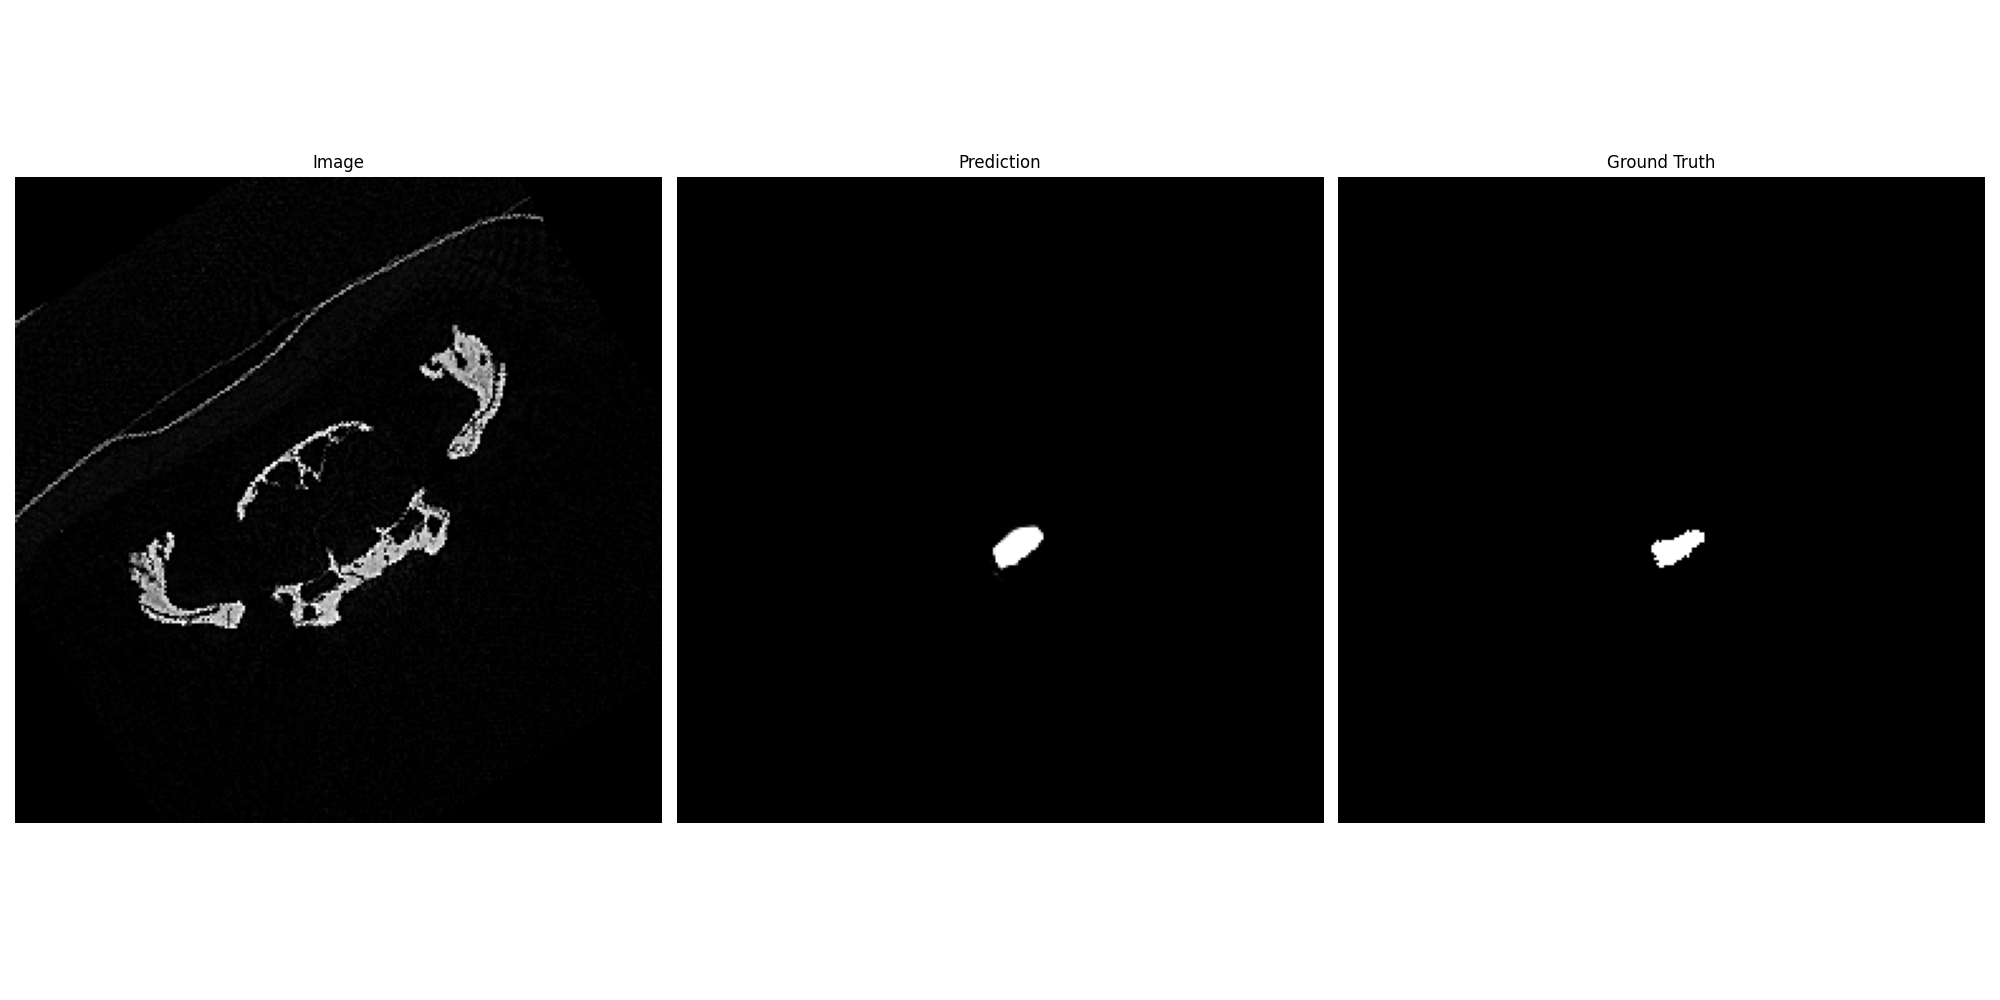
\includegraphics[width=0.99\textwidth]{images/results/prediction2.png}
    \caption{Another example of prediction}
    \label{fig::Prediction2}
\end{figure}
\begin{figure}[!htb]
    \centering
    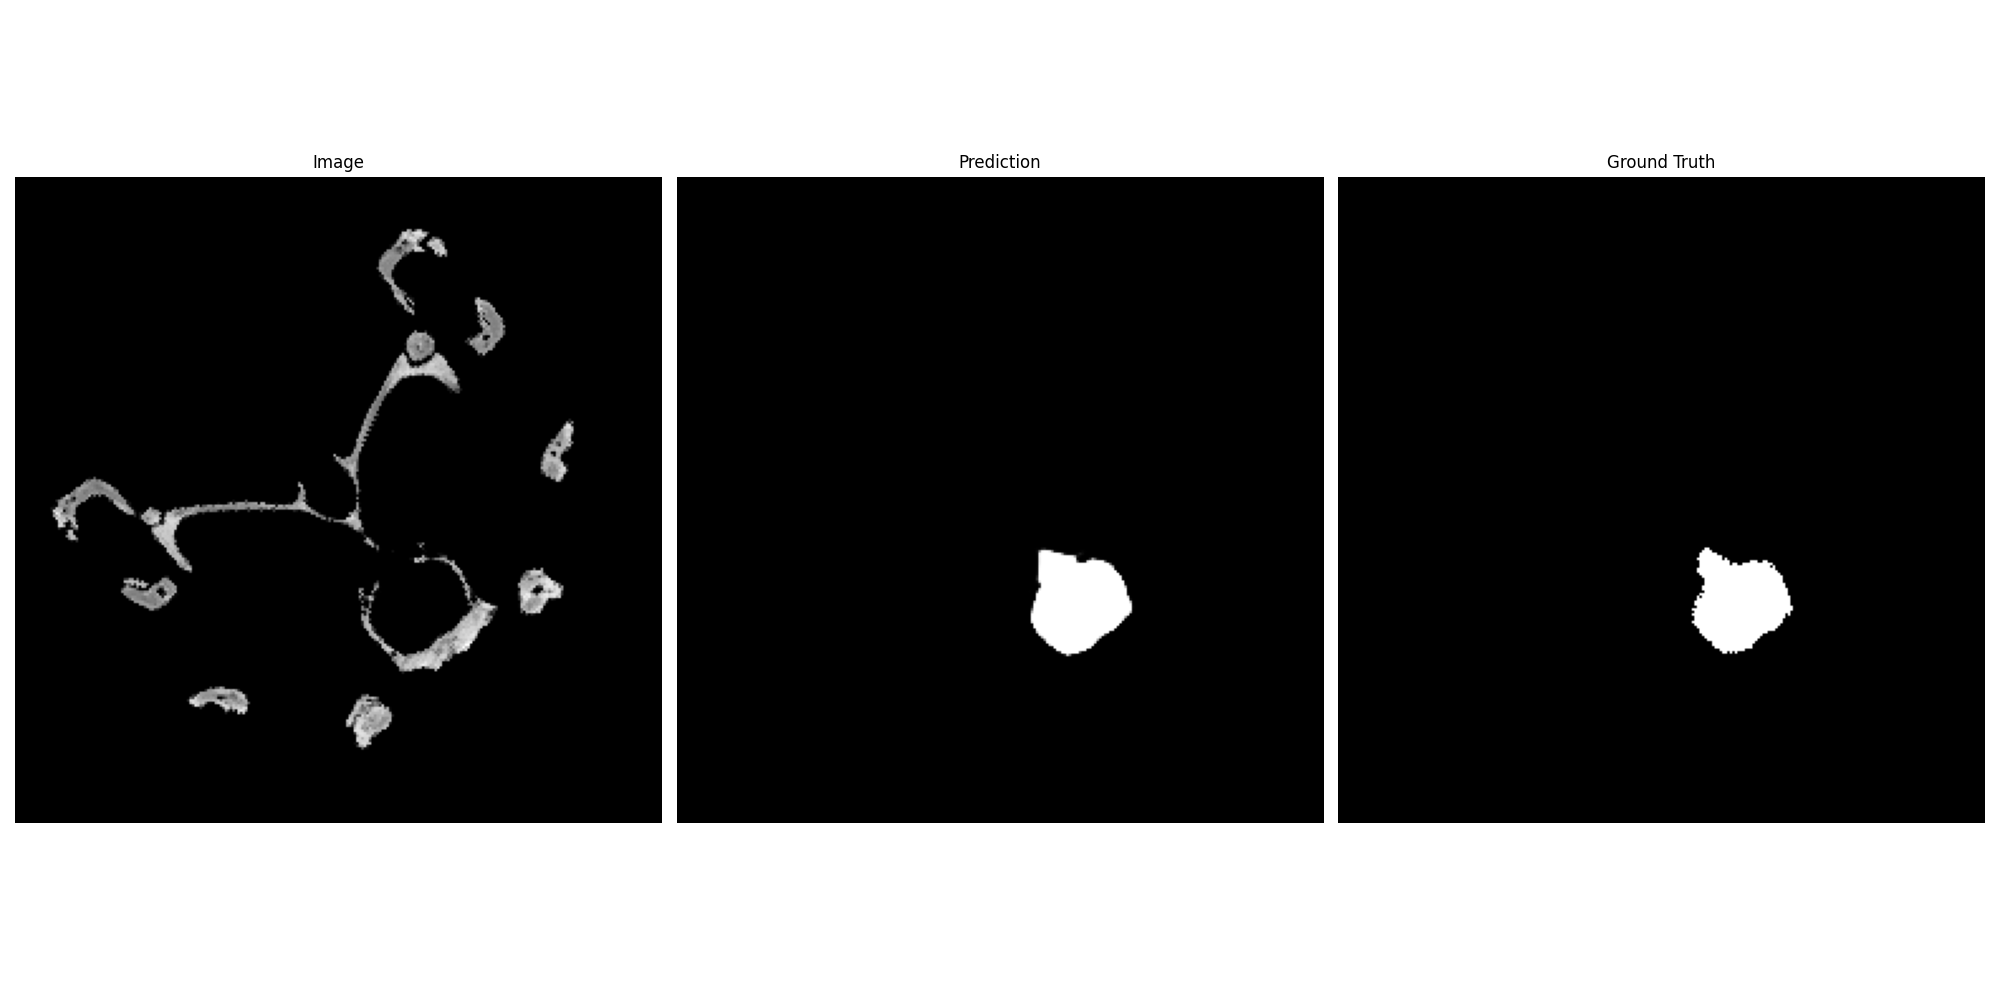
\includegraphics[width=0.99\textwidth]{images/results/prediction3.png}
    \caption{Yet Another example of prediction}
    \label{fig::Prediction3}
\end{figure} % optional
\end{document}

